\documentclass[border=3pt]{standalone}
% Preâmbulo compartilhado pelos diagramas TikZ da aula 4 de Navegação (Representação de Mapas)
\usepackage[T1]{fontenc}
\usepackage[utf8]{inputenc}
\usepackage{lmodern}
\usepackage{amsmath}
\usepackage{xcolor}
\usepackage{tikz}
\usetikzlibrary{arrows.meta,angles,quotes,decorations.pathmorphing,decorations.pathreplacing,calc,
                positioning,shapes.geometric,shapes.misc,backgrounds,fit,
                math}

% Paleta (mesma dos SVGs originais)
\definecolor{dblue}{HTML}{2A5B8C}
\definecolor{dorange}{HTML}{B3541E}
\definecolor{dgreen}{HTML}{4A7C59}
\definecolor{dred}{HTML}{9C4B4B}
\definecolor{dcream}{HTML}{F4F1EA}
\definecolor{dshade}{HTML}{DDD7C9}

% Função gaussiana (não normalizada por padrão de escala visual)
\pgfmathdeclarefunction{gauss}{3}{%
  \pgfmathparse{1/(#3*sqrt(2*pi))*exp(-((#1-#2)^2)/(2*#3^2))}%
}

% Estilos comuns (prefixo d... para não colidir com chaves internas do pgf)
\tikzset{
  >={Stealth[length=2mm]},
  dguide/.style={gray!55, dashed, line width=0.4pt},
  daxis/.style={gray!60, line width=0.7pt, ->},
  dbody/.style={fill=black!3, draw=black!80, line width=1pt},
  dacc/.style={draw=dblue, line width=1pt},
  dlbl/.style={black!55, font=\small},
  dsub/.style={black!45, font=\footnotesize},
  dstate/.style={circle, draw=black!80, fill=dcream, line width=1pt,
                 minimum size=17mm, font=\large, inner sep=1pt},
  dobs/.style={circle, draw=black!80, fill=dshade, line width=1pt,
               minimum size=14mm, font=\large, inner sep=1pt},
  dbox/.style={rounded corners=2pt, draw=black!80, fill=dcream, line width=1pt,
               align=center, inner sep=6pt},
  dop/.style={circle, draw=black!80, fill=white, line width=1pt,
              minimum size=6mm, inner sep=0pt, font=\small},
  dtrans/.style={->, dblue, line width=1pt},
  dmeas/.style={->, dorange, line width=1pt},
  dcurve/.style={line width=1pt, dblue},
  dcurveb/.style={line width=1.4pt, dorange},
}

\begin{document}
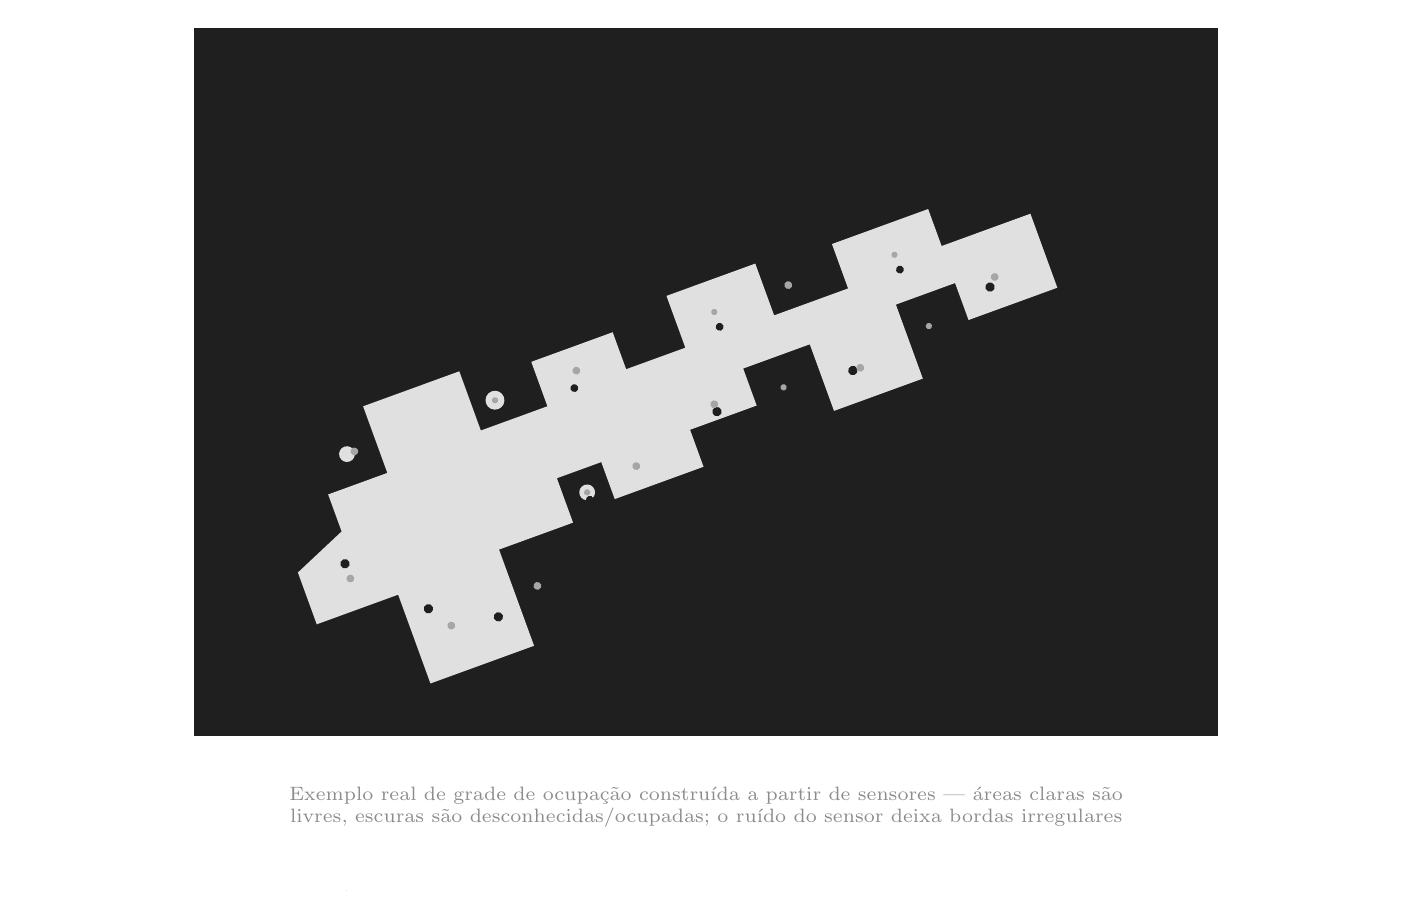
\begin{tikzpicture}[x=1cm,y=1cm]

  \fill[black!88] (0,0) rectangle (13,9);

  \begin{scope}[rotate around={20:(6.5,4.5)}]
    % silhueta principal: corredor com salas alternadas, contorno serrilhado
    \fill[black!12]
      (0.8,4.0) -- (0.8,3.3) -- (1.9,3.3) -- (1.9,2.1) -- (3.3,2.1) -- (3.3,3.4)
      -- (4.3,3.4) -- (4.3,4.0) -- (4.9,4.0) -- (4.9,3.5) -- (6.1,3.5) -- (6.1,4.0)
      -- (7.0,4.0) -- (7.0,4.5) -- (7.9,4.5) -- (7.9,3.6) -- (9.1,3.6) -- (9.1,4.6)
      -- (9.9,4.6) -- (9.9,4.1) -- (11.1,4.1) -- (11.1,5.1) -- (9.9,5.1) -- (9.9,5.6)
      -- (8.6,5.6) -- (8.6,5.0) -- (7.6,5.0) -- (7.6,5.7) -- (6.4,5.7) -- (6.4,5.0)
      -- (5.6,5.0) -- (5.6,5.5) -- (4.5,5.5) -- (4.5,4.9) -- (3.6,4.9) -- (3.6,5.7)
      -- (2.3,5.7) -- (2.3,4.8) -- (1.5,4.8) -- (1.5,4.3) -- cycle;

    \draw[black!12, line width=0pt] (0,0) rectangle (0,0); % placeholder

    % pequenas reentrâncias/saliências de ruído ao longo da borda
    \foreach \p/\s in {(1.2,3.6)/0.12,(2.6,2.7)/0.14,(4.6,3.7)/0.10,(5.5,3.7)/0.11,
                       (6.6,4.2)/0.12,(8.4,4.0)/0.13,(10.5,4.6)/0.12,(9.2,5.3)/0.11,
                       (7.0,5.3)/0.10,(5.0,5.2)/0.11,(3.9,5.2)/0.12,(1.9,5.2)/0.10} {
      \fill[black!12] \p circle (\s);
    }
    \foreach \p/\s in {(1.4,3.9)/0.06,(2.2,3.0)/0.06,(3.0,2.6)/0.06,(4.6,3.6)/0.05,
                       (6.5,4.1)/0.06,(8.3,4.0)/0.06,(10.3,4.4)/0.06,(9.3,5.0)/0.05,
                       (6.9,5.1)/0.05,(4.9,5.0)/0.05,(2.0,5.0)/0.05} {
      \fill[black!88] \p circle (\s);
    }

    % textura interna: pequenas manchas mais claras/escuras (ruído do sensor)
    \foreach \p/\r in {(1.4,3.7)/0.05,(2.4,2.7)/0.05,(3.6,2.8)/0.05,(4.6,3.7)/0.04,
                       (5.3,3.8)/0.05,(6.5,4.2)/0.05,(7.4,4.1)/0.04,(8.4,4.0)/0.05,
                       (9.4,4.2)/0.04,(10.4,4.5)/0.05,(9.3,5.2)/0.04,(7.9,5.3)/0.05,
                       (6.9,5.3)/0.04,(5.0,5.2)/0.05,(3.9,5.2)/0.04,(2.0,5.2)/0.05} {
      \fill[black!35] \p circle (\r);
    }
  \end{scope}

  \node[dsub, font=\scriptsize, align=center, text width=17cm] at (6.5,-0.9)
     {Exemplo real de grade de ocupação construída a partir de sensores --- áreas claras são livres, escuras são desconhecidas/ocupadas; o ruído do sensor deixa bordas irregulares};

\end{tikzpicture}
\end{document}
